\documentclass[aspectratio=169,11pt]{beamer}

\usetheme{Madrid}
\usecolortheme{default}
\usefonttheme{professionalfonts}
\setbeamertemplate{navigation symbols}{}
\setbeamertemplate{footline}[frame number]

\usepackage{amsmath, amssymb, booktabs, graphicx}
\graphicspath{{../../assets/figures/}{assets/figures/}}

\title{Dynamic Labor Supply and Lifecycle Responses}
\subtitle{Labor I --- Week 3}
\author{Teaching deck draft}
\date{}

\begin{document}

\begin{frame}
  \titlepage
\end{frame}

\begin{frame}{Central question and motivation}
\begin{itemize}
    \item How do labor-supply choices change once workers can shift work across time instead of choosing hours one period at a time?
    \item Week 2's static condition survives, but now assets, anticipation, and lagged choices matter for what an estimate means.
    \item Dynamic evidence is useful because temporary shocks, permanent shocks, and lifecycle changes do not identify the same object.
\end{itemize}
\end{frame}

\begin{frame}{Dynamic labor-supply problem}
\[
\max_{\{c_t,h_t,a_{t+1}\}_{t=0}^T}
\sum_{t=0}^T \beta^t u(c_t,\bar h-h_t)
\quad \text{s.t.} \quad
a_{t+1} = (1+r)a_t + y_t + w_t h_t - T_t(w_t h_t,y_t) - c_t
\]

\begin{itemize}
    \item Current work changes both current resources and future feasible choices.
    \item The shadow value of wealth is therefore an intertemporal state variable.
\end{itemize}
\end{frame}

\begin{frame}{Intratemporal condition and Frisch interpretation}
\[
\frac{u_{\ell,t}(c_t,\ell_t)}{u_{c,t}(c_t,\ell_t)}
= w_t \bigl(1-\tau_t^m\bigr),
\qquad \ell_t = \bar h - h_t
\]

\begin{itemize}
    \item The Frisch elasticity holds fixed the marginal utility of wealth.
    \item That makes it an intertemporal substitution object, not a generic policy elasticity.
    \item Permanent wage changes mix substitution and wealth effects, so they are not clean Frisch experiments.
\end{itemize}
\end{frame}

\begin{frame}{Temporary versus permanent wage changes}
\begin{center}
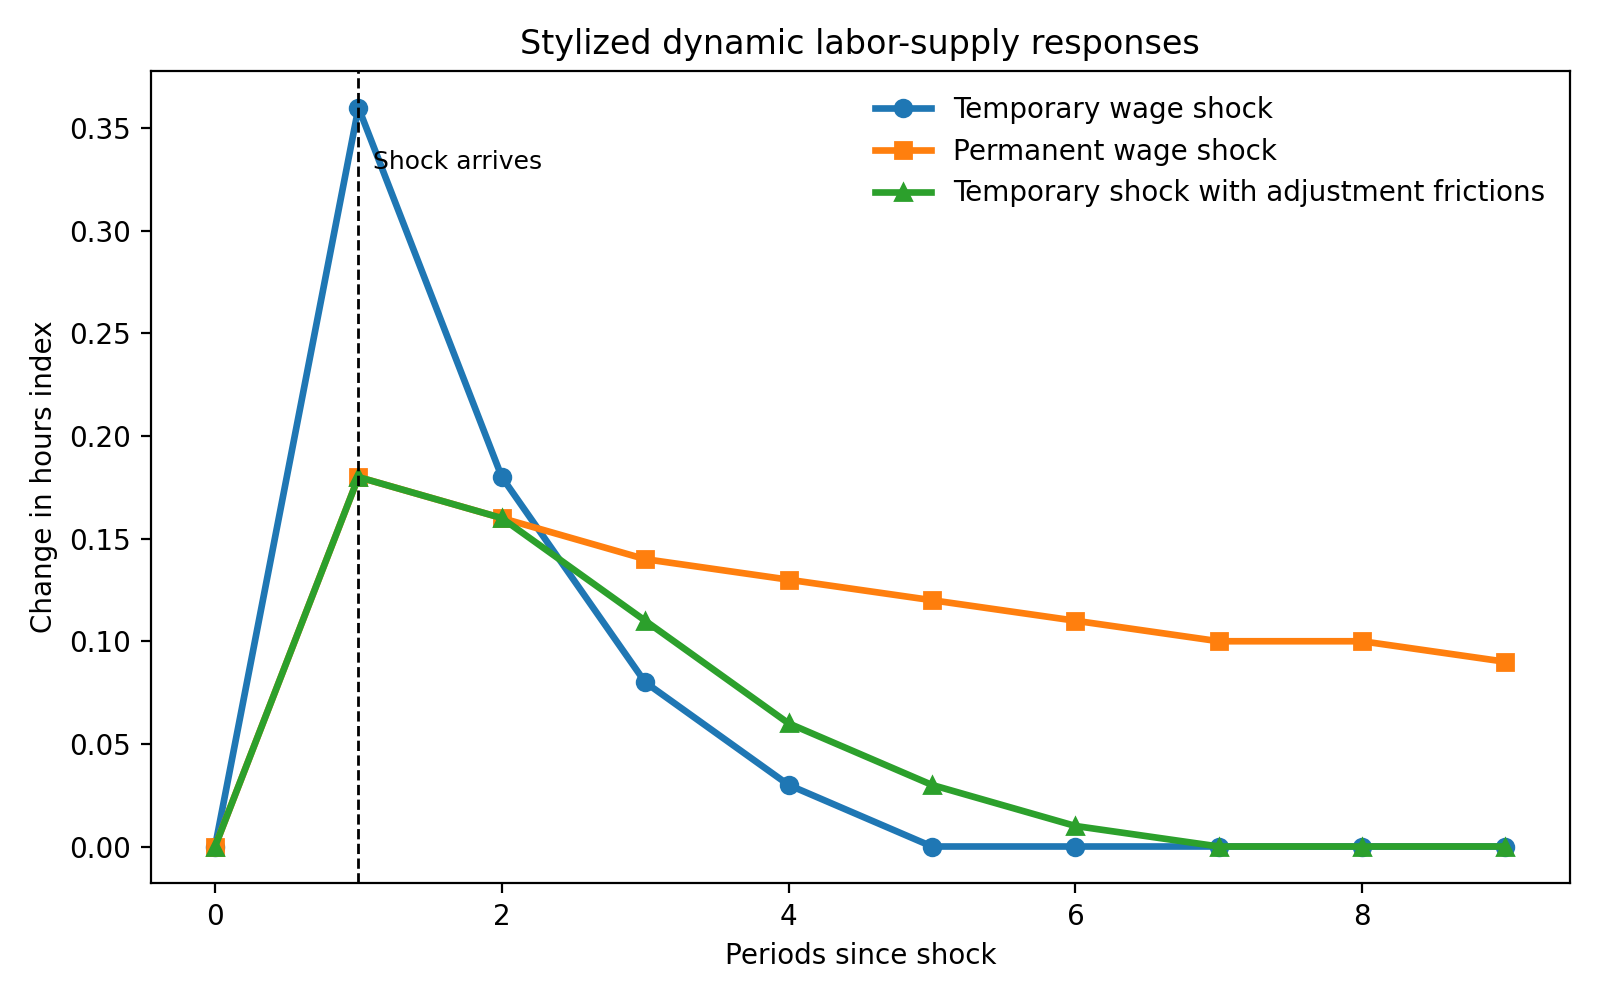
\includegraphics[height=0.74\textheight,keepaspectratio]{03-temporary-permanent-shock-responses.png}
\end{center}
\end{frame}

\begin{frame}{Why lifecycle profiles matter}
\begin{center}
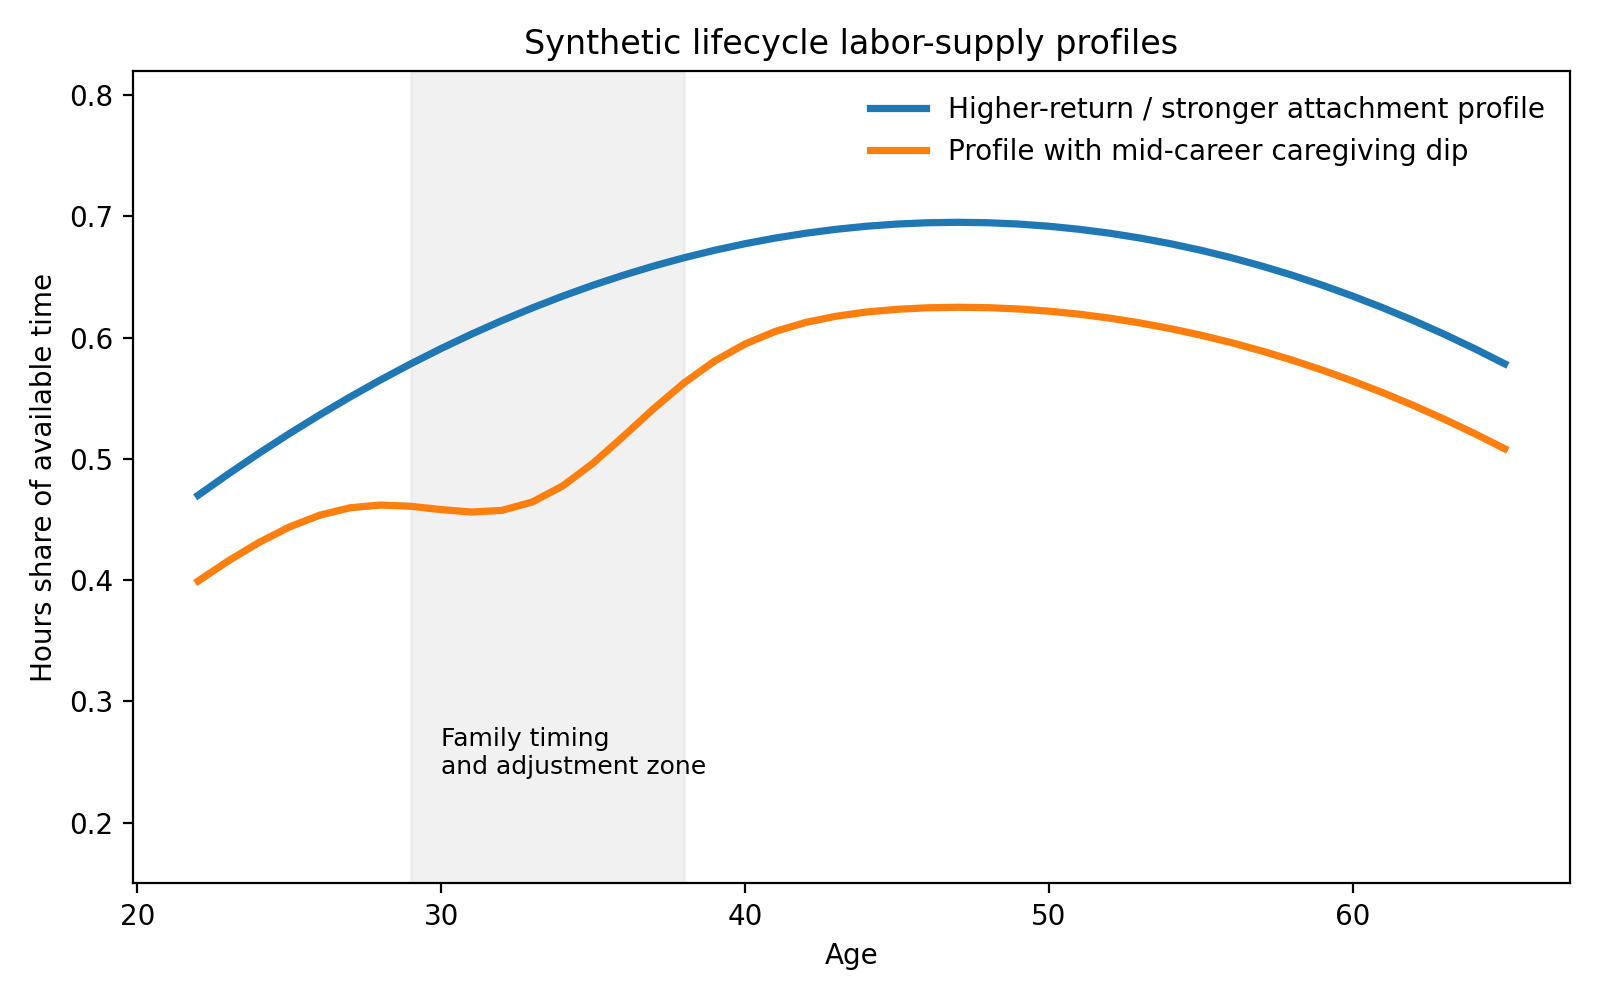
\includegraphics[height=0.74\textheight,keepaspectratio]{03-lifecycle-labor-supply-profiles.png}
\end{center}
\end{frame}

\begin{frame}{Lifecycle logic}
\begin{itemize}
    \item Hours profiles over age are equilibrium objects shaped by wages, family timing, health, and retirement.
    \item Human-capital accumulation means current hours can raise future wages.
    \item That is why Week 3 naturally feeds Week 4: labor supply and skill accumulation are already intertwined.
\end{itemize}
\end{frame}

\begin{frame}{Empirical design map}
\small
\begin{tabular}{p{0.28\linewidth} p{0.28\linewidth} p{0.31\linewidth}}
\toprule
Design & Main variation & Object learned \\
\midrule
Randomized temporary wage variation & Short-run exogenous pay shift & Intertemporal substitution / Frisch-like response \\
Panel wage-hours variation & Within-worker changes over time & Dynamic reduced-form response \\
Tax timing or reform design & Timing or slope of net-of-tax schedule & Horizon-specific labor-supply response \\
Lifecycle structural model & Joint restrictions on wages, hours, savings, family states & Parameters for richer counterfactual policy analysis \\
\bottomrule
\end{tabular}
\end{frame}

\begin{frame}{Persistence and adjustment costs}
\[
\tilde u_t
= u(c_t,\bar h-h_t) - \Phi(h_t-h_{t-1}),
\qquad
\Phi(h_t-h_{t-1}) = \frac{\kappa}{2}(h_t-h_{t-1})^2
\]

\begin{itemize}
    \item Small observed short-run responses need not imply small desired reoptimization.
    \item Adjustment costs, participation costs, and rigid schedules can smooth the measured response.
    \item This is the bridge from micro estimates to the broader elasticity debate.
\end{itemize}
\end{frame}

\begin{frame}{What the Week 3 lab identifies}
\begin{itemize}
    \item Reproduce: a bounded response to randomized temporary wage variation in the spirit of Fehr and Goette.
    \item Diagnose: ask whether the response is best read as intertemporal substitution or a broader labor-supply object.
    \item Transfer: compare the same temporary incentive under low and high adjustment-cost environments.
\end{itemize}
\end{frame}

\begin{frame}{Bridge to Week 4}
\begin{itemize}
    \item If current work raises future wages, labor supply already contains human-capital investment.
    \item Lifecycle differences in hours can therefore reflect changing returns to experience, not only changing tastes.
    \item Week 4 makes that implicit investment margin explicit.
\end{itemize}
\end{frame}

\begin{frame}{Takeaways}
\begin{itemize}
    \item Dynamic labor supply is about timing, not just levels.
    \item Temporary and permanent shocks identify different objects.
    \item The Frisch elasticity is conditional on the intertemporal shadow value of wealth.
    \item Persistence and adjustment frictions are part of the estimand, not a nuisance afterthought.
\end{itemize}
\end{frame}

\end{document}
